%Chapter 2

\chapter{Apprentissage profond} % Main chapter title

%\label{Chapter2} % For referencing the chapter elsewhere, use \ref{Chapter1} 

%\lhead{Chapter 2. \emph{Apprentissage profond}} % This is for the header on each page - perhaps a shortened title

Quelles sont les limites de l'intelligence des ordinateurs? C'est une question toujours ouverte, même en étant l'une des toutes premières à être posées depuis l'invention des ordinateurs. 

On peut trouver dans un dictionnaire que l'apprentissage est: "La capacité d'acquérir et d'appliquer les connaissances". Et si les ordinateurs développaient la capacité d'apprendre?

\section{Apprentissage automatique:}



La tâche de l'apprentissage automatique est de concevoir un algorithme d'apprentissage fiable pouvant être utilisé pour différents problèmes dans des domaines différents. Son utilisation pourrait couvrir plusieurs tâches très distinctes tel que la prévision du marché boursier, la découverte de motifs dans les données scientifiques ou même la reconnaissance d'objets dans les images.

En fait, à travers l'exploration du processus d'apprentissage du cerveau, les scientifiques ont fait l'hypothèse qu'il pourrait y avoir un algorithme d'apprentissage unique utilisé pour une variété de tâches.

Une expérience a été conçue par [Roe et al. 92] au Département du MIT de Brain and Cognitive Sciences, où ils ont coupé le lien entre l'oreille et le cortex auditif, et y ont relié les nerfs optiques (Le cortex auditif étant la partie du cerveau responsable des processus qui traitent l'information auditive capturé par l'oreille). Ils ont découvert que le cortex auditif a appris à traiter les données optiques. En d'autres termes, la partie du cerveau qui une fois a appris à entendre, maintenant apprend à voir.

\begin{figure}[H]
	\centering
		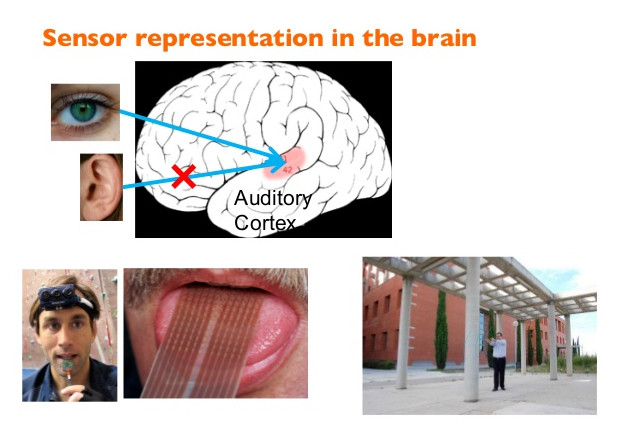
\includegraphics[width=5in]{Figures/OneLearningAlgoAndreNg.jpg}
	\caption[An Electron]{Représentation des sensations dans le cerveau.}
	\label{fig:Electron}
\end{figure}


La même expérience a été reproduite avec succès à plusieurs reprises et avec des configurations différentes (différentes régions du cerveau, des espèces différentes, etc.) qui ont conduit aux mêmes résultats.


L'apprentissage automatique vise à concevoir ce genre d'algorithme. L'objectif est de trouver des modèles dans les données utilisées pour l'apprentissage, et les utiliser pour construire des modèles mathématiques pour faire des prédictions pour de nouvelles données.

\section{Concept de base de l'apprentissage:}


D'après la définition de [Mit et al. 97] "Un programme informatique apprend d'une expérience \textit{E} à effectuer une tâche \textit{T} si sa performance \textit{P} mesurée pour cette tâche \textit{T} s'améliore avec l’expérience \textit{E}."

La description de ce que les éléments \textit{E},\textit{T} et \textit{P} , comme donné dans [Goo et al. 16] est très claire et peut être vue comme suit :

\subsection{Les tâches \textit{T}:} 
L'apprentissage automatique intervient dans des tâches où l'algorithmique classique est incapable de donner des résultats satisfaisants, ou prendrait simplement trop de temps. Ces tâches peuvent être par exemple des tâches de :

\textbf{Classification:} Où le programme doit trouver la classe $c \in C$ à laquelle une entrée \textit{X} appartient. En d'autres termes, on cherche à apprendre une fonction $F : \mathbb{R}^{n} \rightarrow C$ (C étant un ensemble discret ${1..k}$).

\textbf{Classification avec manque de données:} Elle rajoute un niveau de difficulté à la tâche de classification en supposant que certaines données peuvent être manquantes. Le classifieur devrait dans ce cas apprendre plusieurs fonctions avec différents sous ensembles des attributs de l'entrée \textit{X}.

\textbf{Régression:} Cette tâche ressemble à une classification, sauf que le résultat qui fut la classe devient une valeur numérique, et l'espace de sortie devient continu. Nous cherchons donc à trouver une fonction $F : \mathbb{R}^{n} \rightarrow \mathbb{R}$.

\textbf{Transcription:} Elle ressemble encore à la classification, sauf que ce que nous cherchons en sortie au lieu d’être une classe, est une séquence de symboles. Comme par exemple la traduction d'une phrase dans une autre langue.

\textbf{Détection d'anomalie:} Où le programme examine constamment une série d’événements ou de données d'entrée et signal s'il trouve quelque chose d'inhabituel. Une de ses applications est la détection de fraude dans l'utilisation de carte de crédit.

\textbf{Débruitage:} Permet d'apprendre à "nettoyer" une entrée \textit{x'} qui peut-être corrompue par un certain processus de corruption et retourner l'entrée originale \textit{x} .


\subsection{Les mesures de performance \textit{P}:}
La mesure de performance sert d'outil pour déterminer si un programme effectue bien la tâche \textit{T} souhaitée. La mesure diffère d'une tache à une autre. 

La mesure se fait sur les données dont ont dispose et qu'on utilise pour l'apprentissage, mais aussi sur une partie de données mise de coté (non utilisée pour l'apprentissage). Le plus important étant de savoir si le programme retournera de bons résultats sur des instances qu'il n'a jamais rencontré.   

Plusieurs mesures de performance existent pour les tâches de classification, la mesure de précision est généralement utilisée (nombre d'exemple bien classé sur le nombre total d'exemples). Mais pour d'autres tâches, le choix de la mesure peut être plus difficile à faire.

\subsection{L’expérience \textit{E}:}
L'expérience peut être définie par un scénario que le programme est sensé suivre durant son apprentissage, ce scénario est appelé un algorithme d'apprentissage.

Ces algorithmes se divisent en trois grandes catégories:
\textbf{Non-supervisé:} Le programme reçoit un ensemble de données (des exemples) qu'il se doit d'étudier pour satisfaire une tâche précise qui revient soit à minimiser un coût (pour augmenter la performance), soit à trouver des caractéristiques liants les attributs des exemples pour diviser ces derniers en catégories, par exemple: clustering, PCA, etc.

\textbf{Supervisé:} Le résultat du traitement de chaque exemple est connu. À chaque fois que le programme retourne la valeur de la fonction à apprendre, cette dernière est comparée avec la valeur juste (connue), si elle est conforme le programme est sur la bonne voie, sinon des modifications sur les paramètres appris doivent être effectuées.(ex: Réseaux de neurones, SVM, arbre de décision ... etc).

\textbf{Apprentissage par renforcement:} est un type différent des deux premiers dans le sens où le programme est perçu comme un agent qui interagie dans un environnement et qui reçoit des feedbacks lui permettant d’établir une "politique" qui vise à maximiser ses "gains" ou "récompenses", par exemple: Q-learning.


\subsection{Exemple d'algorithme d'apprentissage: Réseaux de neurones :}
Une des techniques les plus utilisées pour l'apprentissage automatique supervisé (et aussi pour le non-supervisé) est les réseaux de neurones (Perceptron multicouche). 
Un réseaux de neurones artificiel essaye d'imiter le fonctionnement des réseaux de neurones biologiques. Appelé aussi perceptron multicouche, ces derniers sont comme leur nom l'indique, formés de plusieurs couches de neurones. La première est la couche d'entrée, celles du milieu sont les couches cachées et la dernière est la couche de sortie.
Si on prend par exemple un réseau à une seule couche cachée:


\begin{figure}[H]
	\centering
		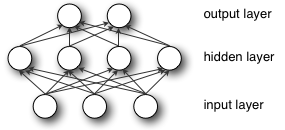
\includegraphics[width=3in]{Figures/mlp.png}
	\caption[An Electron]{Réseau de neurones à une seule couche cachée.}
	\label{fig:Electron}
\end{figure}

Chaque neurone prend en entrée un vecteur, le multiplie par un poids \textit{w}, et y rajoute un biais \textit{b}. Le résultat sera ensuite entré dans une fonction d'activation \textit{s} (qui peut être par exemple: $Sigmoide(x) = 1/(1+e^{x})$ ), et \textit{G} étant une fonction d'activation de la couche de sortie, cette dernière est choisie selon la tâche voulue (par exemple: regréssion, classification, etc.).
Tout le processus est schématisé par un calcul matriciel. L’expression de la fonction \textit{f} que nous essayerons d'apprendre serait :

$$f(x) = G( b^{(2)} + W^{(2)}( s( b^{(1)} + W^{(1)} x)))$$

Avec \textit{x} étant le vecteur d'entrée et \textit{w1}, \textit{ b1}, \textit{w2} et \textit{b2} étant les matrices de poids et vecteur biais entre respectivement, la couche d'entrée et la couche cachée, et entre la couche cachée et la couche de sortie. C'est ces paramètres qui seront appris.
Pour pouvoir se rapprocher de la fonction souhaitée, les paramètres à apprendre (\textit{w1}, \textit{ w2}, \textit{b1} et \textit{b2}) seront changés à chaque itération grâce à différents algorithmes, le plus utilisé étant l'algorithme rétropropagation du gradient (backward propagation of errors). 
Ayant le résultat souhaité et le résultat retourné, l'idée est de définir une fonction "coût" (l'inverse de la performance) qui décrira à quelle fonction \textit{f} serait-elle loin de ce qui est recherché. Ensuite dériver \textit{f} en fonction de chaque paramètre, et changer ces derniers dans le sens qu'il faut (rajouter à sa valeur, ou en soustraire).

Comme mentionné précédemment, l'apprentissage d'une tâche \textit{T} est sensé permettre une application de ce qui a été acquis sur de nouvelles données, ceci est appelé la généralisation.
La généralisation d'un apprentissage peut faire face à plusieurs problèmes, les plus majeurs sont:

\textbf{Le sur-apprentissage:} Quand le programme retourne de bon résultats sur les données d'apprentissage, mais n'arrive pas à généraliser sur des données qu'il n'a jamais rencontré auparavant.

\textbf{Le sous-apprentissage :} Dans le cas où le programme n'arrive même pas à trouver un modèle qui satisfait les données de l'apprentissage.


\begin{figure}[H]
	\centering
		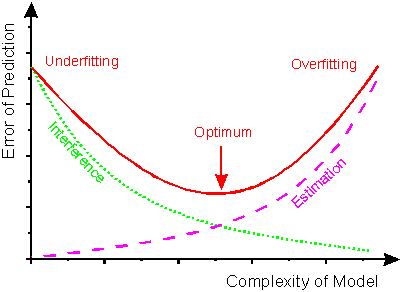
\includegraphics[width=3in]{Figures/image024.png}
	\caption[An Electron]{Sur-apprentissage et sous-apprentissage}
	\label{fig:Electron}
\end{figure}

\section{Introduction à l'apprentissage profond}

L'apprentissage profond est composé de deux mots: apprentissage et profond. La première partie réfère au fait que ce soit un concept d'apprentissage automatique, et la deuxième partie: profond, réfère à sa structure.

Principalement en raison de la faible puissance de calcul des machines, les algorithmes d'apprentissage n'étaient pas très complexes. Mais grâce à l'évolution exponentielle de la puissance de traitement (loi de Moore) de nouvelles perspectives ont été mises en lumière.
Depuis 2010, l'utilisation de la puissance des GPUs pour les calcules est devenue disponible pour le grand public, les scientifiques sont en mesure d'effectuer efficacement des calculs parallèles sur de très grosses matrices, et donc, ils ont réussi à élargir leurs modèles pour atteindre de manière significative de meilleures performances.


Le deep learning permet de développer des approches d'apprentissage automatique de plus en plus profondes (plus volumineuses et donc plus complexes) mais il permet aussi une très grande flexibilité pour combiner plusieurs techniques. Pourtant, beaucoup de problèmes restent à être réglés. Un des plus gros étant la soi-disant curse of dimentionality (la malédiction de la dimensionnalité). En fait, les données en entrée à un algorithme d'apprentissage sont de haute dimensionnalité. Une image par exemple, est une matrice de milliers, ou peut-être de millions de pixels, chacun peut prendre des centaines de valeurs différentes. Si nous prenons par exemple une image de $100 \times 100$, le nombre de configurations distinctes qu'elle peut prendre est:
$256^{3} \times 100 \times 100 = 1 677 721 600$.

Cet espace de valeurs est évidemment trop large pour pouvoir en couvrir même une fraction. Mais le problème serait plus à propos de fonctions de hautes variations que nous essayons de reproduire. En fait, si la fonction n'est pas trop complexe, même dans des dimensions élevées, quelques exemples pourraient être suffisants pour l'apprentissage de sa représentation, et si la fonction cible a beaucoup de variations, nous aurons besoin en conséquence de plusieurs exemples d'apprentissage, comme le montre la figure suivante:

\begin{figure}[H]
	\centering
		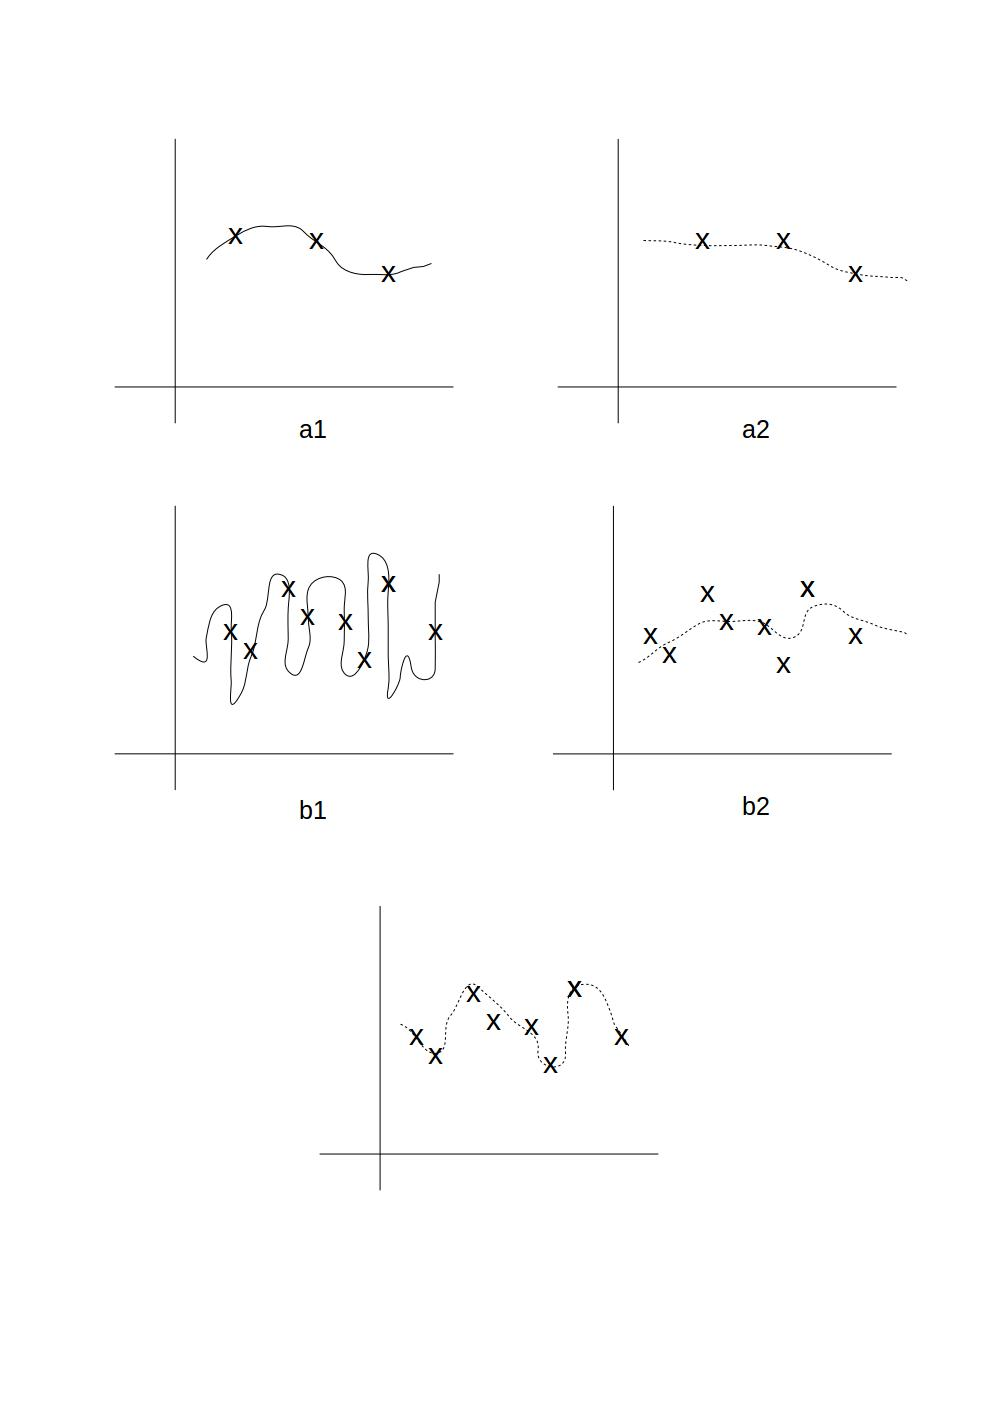
\includegraphics[width=3in]{Figures/highVariation.jpg}
	\caption[FA]{Fonctions d'approximation.}
	\label{fig:Electron}
\end{figure}


Dans l'exemple 1, le graphe (a1) montre une fonction simple que le modèle cherche à approximer, et le graphe (a2) montre le résultat de l'approximation obtenu par le modèle. Ce résultat est satisfaisant malgré le nombre  réduit d'exemples.

Quant à l'exemple 2, le graphe (b1) montre une fonction plus complèxe que celle du graphe (a1), la tâche d'approximation devient plus difficile. Les tentatives du modèle  (représentées respectivement par les graphes (b2) et (b3)) de ne pas passer par tous les exemples, ou de passer par tous les exemples échouent à trouver un résultat satisfaisant dans les deux cas. 

Pour une dimension \textit{D} de donnée en entrée (exemple: age, sexe, etc.) ou sur une variété de dimension D, le nombre de variations peut croître de façon exponentielle avec \textit{D}, d'où résulte le grand nombre d'exemples requis. [Yos 14]

\section{Les Architectures de l'apprentissage profond:}

Bien que le principe des algorithmes d'apprentissage existants est unique (en passant par un tas de données pour trouver des modèles significatifs et construire des modèles mathématiques afin de réaliser une tâche d'apprentissage), pour s'adapter à des objectifs différents, plusieurs concepts et architectures sont appliqués, parmi eux:
 

\subsection{Deep Belief Networks}

Réseaux profond de croyance est une pile de machines de Boltzmann restreintes (RBM) qui se termine généralement avec une unité de classification. Un RBM est un réseaux de neurones à deux-couches (une visible et l'autre cachée) stochastique (l'activation de neurones est probabiliste)

Les DBN sont utilisés pour le pré-apprentissage non-supervisé, pour une meilleure initialisation des poids.



\subsection{Réseau de neurones à convolution}
L'idée a été inspirée du travail de Hubel et Wesley sur le cortex visuelle du chat [Hub et al. 68]. Un réseau de neurones à convolution ou Convolutional Neural Network (ConvNets), vise à émuler le réseau de neurones biologique.
	La mise en œuvre la plus commune d'un réseau de neurones à convolutions est LeNet de [Lec and Wie 98], qui empile différentes couches de convolution et sous-échantillonnage, suivies à la fin d'une multicouche de perceptrons entièrement connectés comme indiqué sur la figure suivante :

\begin{figure}[H]
	\centering
		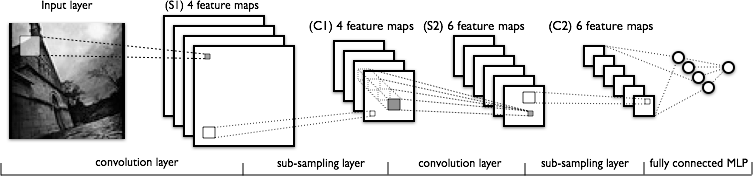
\includegraphics[width=5in]{Figures/Mylenet.png}
	\caption[An Electron]{Exemple de couches de convolution.}
	\label{fig:Electron}
\end{figure}


\subsubsection{La convolution}
La convolution est un terme mathématique, définie comme l'application d'une fonction de façon répétée à travers la sortie d'une autre fonction. Dans ce contexte, il signifie d'appliquer un filtre sur une image en prenant en compte tous les décalages possibles. Comme le montre la figure suivante:


\begin{figure}[H]
	\centering
		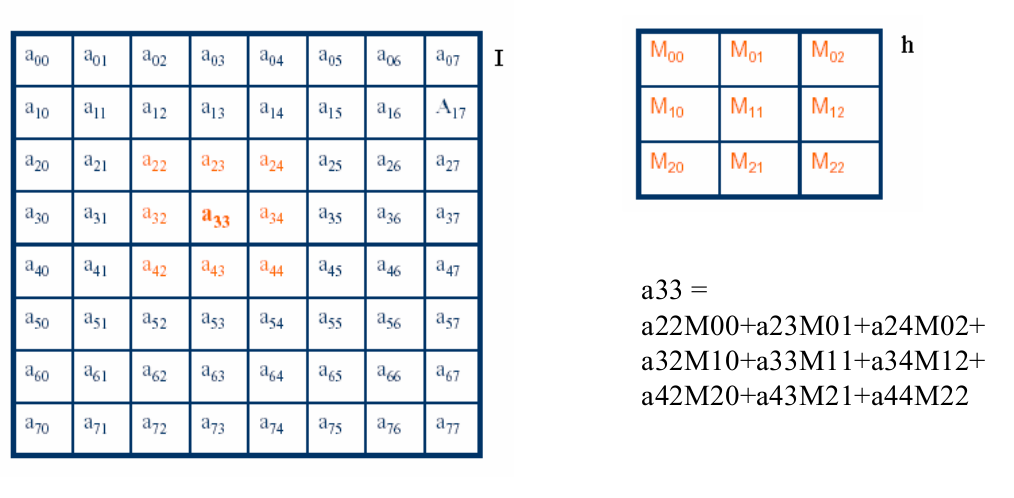
\includegraphics[width=5in]{Figures/convAouat.png}
	\caption[An Electron]{Exemple de convolution}
	\label{fig:Electron}
\end{figure}



Les couches de convolution appliquent simplement des convolutions sur les couches précédentes en utilisant différents filtres. Les poids de chaque filtre sont appris grâce à une rétropropagation (backpropagation).

\subsubsection{Le padding}
Afin de mieux contrôler la taille des images obtenues après l'application d'une convolution sur une image en entrée, on peut utiliser ce qu'on appelle "padding" (remplissage) avant une convolution.
L'une des techniques utilisée pour le padding est le zero-padding, pour cela il suffit de rajouter des zéros aux bords de l'image. Pour un zero-padding de 1, on a le résultat de la figure suivante:

\begin{figure}[H]
	\centering
		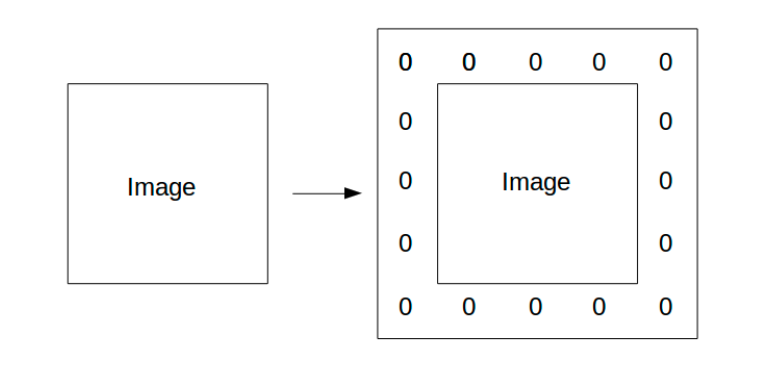
\includegraphics[width=5in]{Figures/zero-padding.png}
	\caption[An Electron]{Application d'un zero-padding sur une image}
	\label{fig:Electron}
\end{figure}

Nous pouvons aussi utiliser le zero-padding pour conserver exactement la taille spatiale d'une image après l'application d'une convolution, de sorte que la largeur d' entrée et de sortie et la longueur sont les mêmes, comme nous le verrons dans le prochain chapitre.


\subsubsection{Le sous-échantillonnage}
Le sous-échantillonnage (ou subsampling) se réfère à la réduction de la taille globale d'un signal. Dans de nombreux cas, comme la compression audio pour les fichiers de musique, le sous-échantillonnage se fait simplement pour la réduction de la taille. 

La méthode de sous-échantillonnage spécifique utilisée dans LeNets est connue comme max-pooling. Cela implique le fractionnement d'une matrice (image) en de petits fragments qui ne se chevauchent pas (plus les fragments sont grands, plus la réduction est importante), et de prendre la valeur maximale dans chaque grille en tant que la valeur dans la matrice réduite. 
Ceci permet, entre autre, l'obtention d'une invariance aux translations. La figure suivante montre un exemple de l'application d'un max-pooling:


\begin{figure}[H]
	\centering
		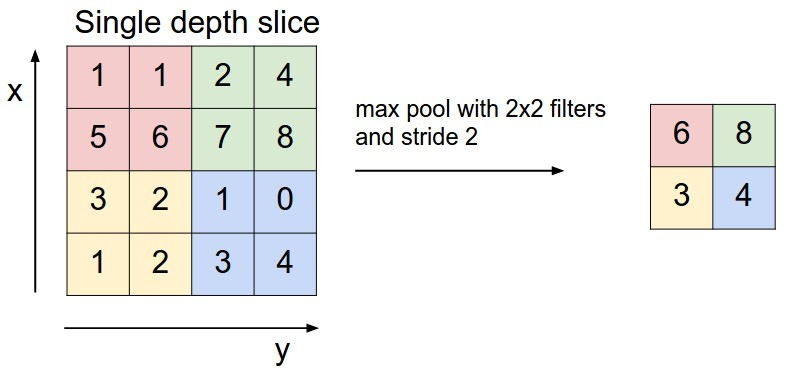
\includegraphics[width=5in]{Figures/maxpool.jpeg}
	\caption[MP]{Exemple max-pooling}
	\label{fig:Electron}
\end{figure}

\subsubsection{Normalisation}
Une des techniques inspirée de la neuroscience computationnelle qui a été utilisée, est l'ajout de couches de normalisation après une couches de convolution. [Kri et al.,12] Néanmoins, la normalisation il semble que ces couches ont un impact très minime et ne sont plus utilisées. Ils ont été dominé par d'autres techniques tels que le "dropout" ainsi qu'une meilleure initialisation des poids des neurones et les algorithmes d'entraînement du réseau.

\subsubsection{Perceptron multicouche entièrement connecté:}

Finalement, après plusieurs couches de mise en commun de convolution et de max-pooling, le traitement final dans le ConvNets se fait via des couches de perceptrons entièrement connectés. Une couche entièrement connectée prend tous les neurones de la couche précédente et les relies à chaque neurone dont elle dispose.

\subsubsection{Dropout}
On applique un dropout lors de la phase d'entraînement d'un réseau de perceptron  multicouche entièrement connecté, précisément lors de la rétropropagation. Son est d'éviter le sur-apprentissage, par exemple pour un taux de dropout de 30\%, la rétropropagation ne s'appliquera pas sur 30\% des neurones d'une couche (ces neurones sont choisis aléatoirement à chaque rétropropagation). Dans ce cas les neurones d'une même couche n'auront pas rencontré (n'apprendront pas) les même exemples (images).

\subsection{Deep Auto-encoders}

Nous avons déjà parlé du problème de curse of dimentionality. Les Autoencoders sont un moyen de résoudre ce problème. Pour cela, ils visent à trouver une représentation compressée des données en entreé.
En d'autres termes, les autoencoders sont un type de réseaux de neurones entraînés d'une manière supervisée par rétropropagation pour reproduire leurs données en entrée après les avoir fait passées à travers des couches cachées de dimension inférieure à celle de l'entrée.

%Une des techniques pour former un "deep autoencoder" de empilant pré-entraîné, et d'ensuite faire une mise au point à la fin avec de la rétropropagation.

Un "deep autoencoder" est construit en empilant un certain nombre de couches de machines de Boltzmann restreintes RBM pré-entraîné. On applique à la fin sur ces couches une mise au point (fine tuning) avec de la rétropropagation (backprop).

Un exemple d'utilisation d'un autoencoder est la recherche d'une représentation de dimension inférieure pour une image. La raison pour laquelle cette représentation pourrait exister est donnée par l'idée suivante :
Si vous essayez de générer une image aléatoire, vous vous  retrouverez très probablement avec une image comme le montre la figure suivante. Peu importe combien de fois vous essayez, vous obtiendrez probablement jamais une image d'un chien, d'une voiture, ou autre chose significative.


\begin{figure}[H]
	\centering
		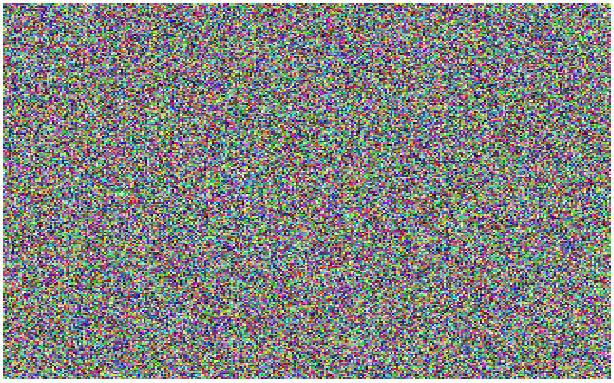
\includegraphics[width=3in]{Figures/randomImageGEn.JPG}
	\caption[An Electron]{Image générée aléatoirement.}
	\label{fig:Electron}
\end{figure}

Ainsi, l'espace des images significatives forme seulement une fraction de l'espace total défini par les valeurs des pixels. L'objectif de l'autoencoder est alors de trouver une représentation d'une image dans cet espace.


\begin{figure}[H]
	\centering
		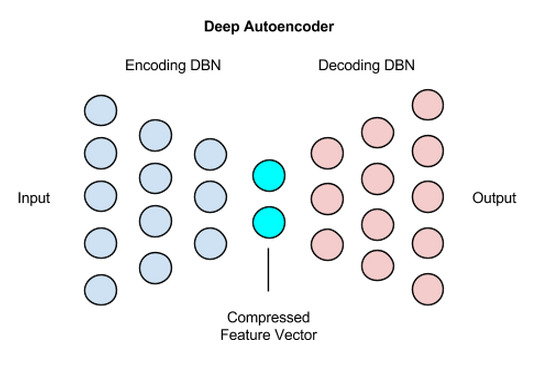
\includegraphics[width=3in]{Figures/deep_autoencoder.png}
	\caption[An Electron]{Exemple d'un modèle d'autoencoder utilisant les DBN.[Site2]}
	\label{fig:Electron}
\end{figure}

\section{Les exploits des techniques d'apprentissage profond [Jia 14]}

L'Apprentissage profond a surperformé les techniques de vision artificielle traditionnelles au cours des dernières années. Dans le concours ImageNet en 2010 (ImageNet est un projet qui a pour but de fournir aux chercheurs une très grande base d'images facilement accessible), le meilleur algorithme de Vision artificielle traditionnelle avait un taux d'erreur de 28,2\%, ce qui signifie qu'il a obtenu de 71.8\% d'images correctes. En 2011, le meilleur algorithme à obtenu un taux d'erreur de 25,8\%. 

	En 2012, cependant, le premier processus d'apprentissage profond est entré dans la compétition et a dépassé en performance toutes les méthodes traditionnelles avec un taux d'erreur de 16,4\%. 
	Après cela, le premier algorithme d'apprentissage profond a ouvert les portes, la compétition a été inondée avec d'autres équipes d'apprentissage profond qui ont atteint un taux d'erreur de 11,7\% en 2013 et 6,7\% en 2014 \textbf{MACHI 7.405\% imagenet website agrees ???? Chap 3}. Le vainqueur de l'édition 2014 a reconnu 93\% des images, un énorme bond en avant surtout par rapport au taux de 72\% atteint par les techniques de vision artificielle traditionnelles en 2010.


\begin{figure}[H]
	\centering
		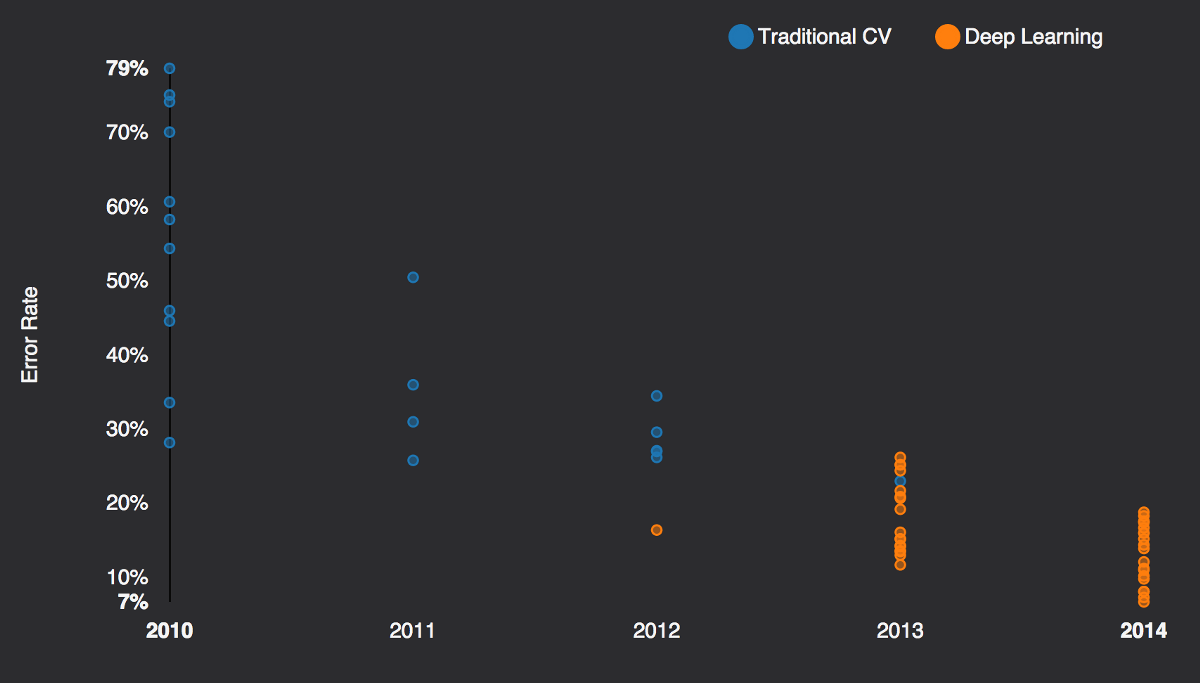
\includegraphics[width=5in]{Figures/clairifaiIMAGENET.png}
	\caption[An Electron]{Résultats du concours d'IMAGEnet.}
	\label{fig:Electron}
\end{figure}